\documentclass{book}
\usepackage[utf8]{inputenc}


\usepackage{natbib}
\usepackage{graphicx}
\usepackage{amsmath,amssymb}
\usepackage{ascmac}
\usepackage{braket}
\usepackage{makeidx}
\makeindex
\usepackage{textcomp}
\usepackage{comment}
\usepackage{authblk}

\begin{document}
\title{Lecture Memo \\ Quantum Mechanics of Light and Matters}
\author{Yasuyuki Ozeki}
\affil{Department of Electrical Engineering and Information Systems \\ The University of Tokyo}
\date{July 25, 2020}

\maketitle
\tableofcontents
\mainmatter

\chapter{Introduction}
Light is regarded as an ensemble of particles called photons. The particle nature of light appears as 'noise' in various applications of light waves such as optical measurement, optical manipulation, and optical communications, leading to the physical limit of the performance or precision achieved by these methods. To enhance 



%光は光子(フォトン)と呼ばれる粒子の集まりである。光が粒子であるということ(量子性)は、光を用いて通信、制御、計測を行う際において雑音として現れ、性能や精度の物理限界を与える。光を用いた計測技術の高精度化・高感度化や光通信の大容量化を図るうえで、その限界を知り、限界を高めていくことは重要であり、そのためには光の量子性に関する理解も欠かせない。また、近年では光の量子性を積極的に活用することで、量子暗号、量子テレポーテーション、量子コンピューティング等の技術の開発も進められている。これらの光の量子性を扱う学問を量子光学という。

%光の検出法には様々な種類があり、それは光の強度を検出する光子数検出法と、光の干渉を用いて光の電界振幅を検出するホモダイン・ヘテロダイン法に大別できる。また、光検出器そのものの雑音の影響を抑制するために、光を検出する前に光増幅を行う場合もある。いずれの場合も、検出に伴う雑音は究極的には量子雑音で制限される。レーザ光など、古典的な波動としての光を用いる場合、光子数を$n$とすると、その信号対雑音比は$n$のオーダーになる。これは、古典的な光を使う限り、どのような検出器、検出方法を用いたとしても超えることのできない壁である。一方、この壁を超える手法として非古典的な光を活用する研究も進められている。これらを統一的に理解する上で、量子光学に関する知識は不可欠である。

%本講義メモは、光の量子雑音の考え方について理解することを目的とする。まず、量子雑音について簡単におさらいしたのち、光の量子論で基本となる放物線ポテンシャルの量子力学と、その記述方法をまとめる。次に、光の光子数が確定した状態や、古典的な状態であるコヒーレント状態など、代表的な光の量子状態についてその性質を議論する。その後、光の計測とそれに伴う量子雑音について述べる。最後に、光増幅に伴う雑音の発生について議論する。

%なお、本講義は電気系の修士1年生を対象としている。

%本講義メモは、2015年度までの菊池和朗教授の講義メモを参考に、2017年度に準備したものです。これまでに多くの学生さんから多数の誤りや分かりにくい点のコメントをいただきました。深く感謝いたします。今後も、お気づきの点があれば\texttt{ozeki@ee.t.u-tokyo.ac.jp}までコメントをお寄せください。


\chapter{Noise in optical measurements}
%本章では、光計測における光の検出法について述べるとともに、光計測において生じる雑音について現象論的に説明する。いくつかの説明は天下りであるが、それらは、後の章で量子光学を用いて説明することとする。
This chapter introduces various detection methods of light and explains noise appearing in each method. Some explanations are phenomenological but they will be explained by quantum optics in later chapters.

\section{Optical measurements}
Figure \ref{fig:photodetection}(a) shows the \textbf{direct detection}. Photodetectors can convert photons to electrons to measure optical power, which is proportional to the number of photons per unit time. 

Fig. \ref{fig:photodetection}(b) shows the \textbf{interferometric detection}, where a beamsplitter (BS) is used to mix the signal light wave to be measured and another light wave called local oscillator (LO) light, and the output light waves of the BS are detected with photodetectors to measure the amplitude of light. When the optical frequencies of signal and LO are the same, the method is called \textbf{homodyne}. When they are different, the method is called \textbf{heterodyne}.

Furthermore, an optical amplifier is often used before photodetection as shown in Fig. \ref{fig:photodetection}(c). This is called \textbf{preamplificatio}. Although not shown in the figure, it is also possible to conduct interferometric detection after preamplification. 

In every case, the output signal of the photodetector contains noise due to various origins such as instability of light sources or optical systems, circuit noise of photodetector(s), and so on. We can somehow reduce these noises, but at last we will see `quantum noise' that cannot be reduced by classical manner. Only quantum optics can control the quantum noise.

Here, before introducing various noise sources, we introduce direct detection, interferometric detection, and preamplification.

\begin{figure}
  \centering
  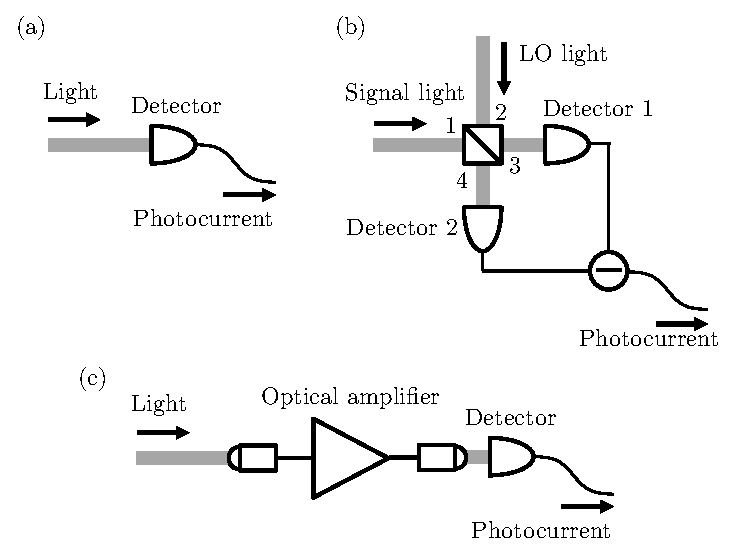
\includegraphics[width=9cm]{fig/1-1_photodetection.eps}
  \caption{Various photodetection methods. (a) Direct detection. (b) Interferometric detection. (c) Optical preamplification with an optical amplifier.}
  \label{fig:photodetection}
\end{figure}


\subsection{Direct detection}
Therefore 
\begin{equation}
	I = \frac{\eta q P}{\hbar \omega}
	\nonumber
\end{equation}

\subsection{Homodyne and heterodyne detection}

\begin{equation}
\begin{aligned}
	a(t) &= \alpha e^{-i(\omega + \Delta \omega)t}\\
  	b(t) &= \beta e^{-i\omega t}
\end{aligned}\label{eq:complex_amplitude}
\end{equation}

\begin{equation}
\begin{aligned}
  a' &= \frac{1}{\sqrt 2}(a - b)\\
  b' &= \frac{1}{\sqrt 2}(a + b)
\end{aligned}\label{eq:BS_complex_amplitude}
\end{equation}

\begin{equation}
  \left( \begin{array}{c}
  	a' \\ b'
  \end{array}
  \right) =
  \frac{1}{\sqrt 2}\left( \begin{array}{r r} 
  	1 & -1 \\ 1 & 1
 \end{array}
	\right)
	\left( \begin{array}{c}
		a \\ b
	\end{array} \right)
	\label{eq:beamsplitter_matrix}
\end{equation}

\begin{equation}
\begin{aligned}
  I_1 &= \frac q \tau |a'|^2 = \frac{q}{\tau}\left|\frac{1}{\sqrt 2} (a - b)\right|^2\\
  I_2 &= \frac q \tau |b'|^2 = \frac{q}{\tau}\left|\frac{1}{\sqrt 2} (a + b)\right|^2
\end{aligned}
\end{equation}

\begin{equation}
\begin{aligned}
  I_2 - I_1 &= \frac{q}{\tau}(ab^* + a^* b)\\
  &= 2qB(\alpha \beta^* e^{-i\Delta\omega t} + \alpha^* \beta e^{i\Delta\omega t})\\
  &= 4qB|\beta|\left\{\mathrm{Re} \  (\alpha e^{-i\phi}) \cos \Delta \omega t + \mathrm{Im} \ (\alpha e^{-i\phi}) \sin \Delta \omega t\right\}
\end{aligned}\label{eq:output_of_balanced_detector}
\end{equation}

Here $B = 1/2\tau$ is the Nyquist frequency, and $\beta = |\beta|e^{i\phi}$.


\section{Noise sources}
\subsection{Shot noise}
\begin{equation}
	p(k) = \frac{\lambda^k e^{-\lambda}}{k!}
\end{equation}

\begin{equation}
\begin{aligned}
	V[p(k)] &= \sum_k{(k-\lambda)^2}p(k)\\
	&= \sum_k{k^2 p(k) - 2\lambda k p(k) + \lambda^2 p(k)} = \sum_k{k^2 p(k) - \lambda^2} \\
	&=\sum_k{k\lambda p(k-1) - \lambda^2} = \lambda\sum_k{\left\{ (k-1)p(k-1) + p(k-1)\right\}}-\lambda^2 \\
	&= \lambda(\lambda + 1) - \lambda^2 = \lambda
\end{aligned}
\end{equation}

\begin{equation}
	\begin{aligned}
		I_{\mathrm{shot}} = q\sqrt{\lambda}/\tau = q\sqrt{\frac{I\tau}{q}}/\tau = \sqrt{\frac{qI}{\tau}}
	\end{aligned}
\end{equation}
\begin{equation}
	\begin{aligned}
		I_\mathrm{shot}=\sqrt{2qIB}
	\end{aligned}
\end{equation}

\begin{equation}
  \mathrm{SNR} = I^2 / I_\mathrm{shot}^2 = I/2qB = 2qB|\alpha |^2/2qB = |\alpha|^2
\end{equation}
where $I=q|\alpha|^2/\tau = 2qB|\alpha|^2$. Since $|\alpha|^2$ corresponds to the number of photons, we can see that the shot-noise limited SNR is equal to the number of photons.


\subsection{Thermal noise}


\subsection{Optical amplifier noise}
\section{Summary}

\chapter{Quantum harmonic oscillators}
\section{Schr\"odinger equation}
\subsection{Wavefunction and energy eigenstates}
\subsection{Fock representation}
\subsection{Position representation}
\subsection{Momentum representation}
\section{Measurement of observables}
\subsection{Expectation value}
\subsection{Expectation of variance}
\section{Multimode quantum states}
\section{Summary}

\chapter{Quantum states and their evolution}
\section{Evolution of quantum states}
\subsection{Schor\"odinger picture}
\subsection{Heisenberg picture}
\section{Unitary transformation of quantum states}
\subsection{Time evolution}
\subsection{Displacement}
\subsection{Mode mixing}
\subsection{Single-mode squeezing}
\subsection{Two-mode squeezing}

\chapter{Quantization of light}
\section{Mode decomposition of electromagnetic waves}
\subsection{Time-frequency mode}
\subsection{Spatial mode}
\subsection{Polarization}
\section{Operator notation of electromagnetic waves}
\section{Summary}

\chapter{Representative quantum states}
\section{Number states}
\section{Superposition states}
\section{Coherent states}
\section{Squeezed states}
\section{Two-mode squeezed states}
\subsection{EPR state}
\section{Summary}

\chapter{Light-matter interaction}
\section{Mode mixing}
\subsection{Beamsplitter}
\subsection{Waveplates}
\subsection{Optical loss}
\subsection{Fourier transform}
\section{Parametric amplification}
\subsection{Squeezing}
\subsection{Spontaneous parametric down conversion}
\subsection{Optical amplification}
\subsection{Raman scattering}
\section{Summary}

\chapter{Measurement of quantum states}
\section{Photodetection}
\section{Homodyne detection}
\section{Heterodyne detection}

\section{Quantum teleportation}

\appendix
\chapter{Appendix}
\section{Bra-ket notation}
\section{Creation and annihilation operators}
\section{Pure states and mixed states}
\section{Wigner function}

\begin{equation}
\begin{aligned}
  \sum_{k=1}^\infty \frac 1 {2^k} &= \frac 1 {2^1} + \frac 1 {2^2} + \frac 1 {2^3} + \dots \\
  &= \frac{1}{2} + \frac{1}{4} + \frac{1}{8} + \dots \\
  &= \frac{\frac 1 2}{1-\frac 1 2} =  1
\end{aligned}
\end{equation}

There is a theory which states that if ever anyone discovers exactly what the Universe is for and why it is here, it will instantly disappear and be replaced by something even more bizarre and inexplicable.
There is another theory which states that this has already happened.

\begin{figure}[h!]
\centering
\includegraphics[scale=1.7]{universe}
\caption{The Universe}
\label{fig:universe}
\end{figure}

%\section{Conclusion}
``I always thought something was fundamentally wrong with the universe'' \citep{adams1995hitchhiker}

\bibliographystyle{plain}
\bibliography{references}
\end{document}
